\chapter{Phân tích và thiết kế hệ thống}
\label{chap:design}

Chương này trình bày quá trình phân tích yêu cầu, kiến trúc tổng quan và thiết kế chi tiết của hệ thống bridge ngang hàng dựa trên intent. Hệ thống được phân tích trên hai trục bổ trợ nhau: trục \textbf{kiến trúc} mô tả các thành phần cấu thành (onchain và offchain), và trục \textbf{thực thi} mô tả cách một intent được phục vụ thông qua mô hình ba lớp Netting Layer, Intent Accelerator Layer và Fallback Bridge Aggregator. Phần cuối của chương trình bày mô hình dữ liệu và các biểu đồ thiết kế chi tiết.

\section{Phân tích yêu cầu}

\subsection{Các tác nhân}

Hệ thống tương tác với các tác nhân sau:

\begin{itemize}
    \item End User: người dùng cuối, tạo và ký intent biểu diễn nhu cầu chuyển tài sản xuyên chuỗi, theo dõi trạng thái và nhận tài sản trên chain đích.
    \item Solver: tác nhân cung cấp thanh khoản và thực thi (fill) intent ở Intent Accelerator Layer; cạnh tranh với các solver khác thông qua cơ chế Dutch auction.
    \item Matching Engine: tác nhân nội bộ của hệ thống, tìm các chu trình bù trừ giữa các intent ở Netting Layer.
    \item Smart Contract on-chain: bao gồm các HTLC Vault triển khai trên các blockchain EVM khác nhau, đóng vai trò khoá tài sản và xác minh các điều kiện thực thi.
    \item Fallback Bridge Aggregator: hệ thống bên thứ ba (ví dụ Chainlink CCIP, Across Protocol) được hệ thống ủy thác khi cả Netting và Accelerator đều không khả thi.
\end{itemize}

% TODO: Use case diagram - actors and use cases of the system.
% Place image at figures/c3/usecase.png and uncomment below.
% \begin{figure}[H]
%   \begin{center}
%   \includegraphics[width=\linewidth]{figures/c3/usecase}
%   \end{center}
%   \caption{Biểu đồ ca sử dụng tổng quan của hệ thống}
%   \label{fig:usecase}
% \end{figure}

\subsection{Yêu cầu chức năng}

Các yêu cầu chức năng được nhóm theo từng module nghiệp vụ:

\paragraph{Quản lý Intent.}

\begin{itemize}
    \item FR-01: Hệ thống cho phép người dùng tạo và submit intent kèm chữ ký số xác thực quyền sở hữu tài sản.
    \item FR-02: Hệ thống quản lý vòng đời intent qua các trạng thái \texttt{QUEUED} $\to$ \texttt{PARTIAL} / \texttt{MATCHED} / \texttt{EXPIRED}.
    \item FR-03: Hệ thống cho phép hủy intent và hoàn trả (refund) tài sản khi quá hạn deadline mà chưa được thực thi.
\end{itemize}

\paragraph{Netting Layer.}

\begin{itemize}
    \item FR-04: Hệ thống mô hình hoá tập intent dưới dạng đồ thị có hướng và tìm các chu trình bù trừ thoả mãn ràng buộc về token, số lượng và deadline.
    \item FR-05: Hệ thống khởi tạo HTLC trên các chain liên quan và settle giao dịch netting một cách nguyên tử.
\end{itemize}

\paragraph{Intent Accelerator Layer.}

\begin{itemize}
    \item FR-06: Hệ thống broadcast intent ra mạng p2p kèm cơ chế incentive tăng dần theo thời gian (Dutch auction).
    \item FR-07: Hệ thống cho phép solver commit và fill intent với mức incentive hiện hành tại thời điểm commit.
\end{itemize}

\paragraph{Fallback Bridge Aggregator.}

\begin{itemize}
    \item FR-08: Hệ thống định tuyến intent qua bridge bên thứ ba khi cả Netting và Accelerator đều không hoàn tất, đồng thời theo dõi và đồng bộ trạng thái cho đến khi giao dịch hoàn tất.
\end{itemize}

\subsection{Yêu cầu phi chức năng}

\begin{itemize}
    \item NFR-01 - Trust-minimization: hạn chế tối đa giả định tin cậy vào bên thứ ba; mọi thao tác giải phóng tài sản phải được kiểm chứng on-chain.
    \item NFR-02 - Tính nguyên tử: với mỗi intent, kết quả phải đảm bảo hoặc tất cả các bên hoàn tất nghĩa vụ, hoặc không bên nào bị thiệt hại.
    \item NFR-03 - Bảo mật: smart contract phải chống các tấn công phổ biến như reentrancy, front-running, replay attack; hệ thống offchain phải xác thực chữ ký và chống Sybil.
    \item NFR-04 - Khả năng phục hồi: tài sản không bị khoá vĩnh viễn; mọi HTLC đều có timelock đảm bảo refund tự động.
    \item NFR-05 - Hiệu năng: độ trễ phù hợp với từng layer --- Netting có thể chấp nhận chờ vài giây, Accelerator yêu cầu đáp ứng gần thời gian thực, Fallback ưu tiên độ tin cậy hơn tốc độ.
    \item NFR-06 - Tối ưu chi phí gas: số lượng giao dịch on-chain được giảm thiểu, ưu tiên matching nội bộ trước khi sử dụng bridge ngoài.
    \item NFR-07 - Non-custodial: hệ thống không nắm giữ tài sản của người dùng tại bất kỳ thời điểm nào. Tài sản chỉ được khoá trong các smart contract escrow (HTLC) với điều kiện giải phóng được kiểm chứng on-chain; trong trường hợp giao dịch không thành công, tài sản sẽ được hoàn trả tự động cho người dùng thông qua cơ chế timelock mà không cần sự can thiệp của bất kỳ bên trung gian nào.
\end{itemize}

\section{Kiến trúc tổng quan hệ thống}

\subsection{Phân tách Onchain và Offchain}

Hệ thống được phân tách rõ ràng thành hai phần lớn: \textbf{onchain} chứa các smart contract chịu trách nhiệm cho các thao tác cần đảm bảo trust-minimized (khoá tài sản, xác minh điều kiện thực thi, settle giao dịch), và \textbf{offchain} chứa các thành phần xử lý intent, matching và điều phối thực thi. 
Việc phân tách này cho phép tận dụng lợi thế của cả hai miền: onchain phụ trách lưu trữ và chuyển giao tài sản một cách an toàn, trong khi offchain phụ trách xử lý order và matching với hiệu năng cao, độ trễ thấp.

% TODO: System architecture diagram - onchain/offchain components.
% Place image at figures/c3/architecture.png and uncomment below.
% \begin{figure}[H]
%   \begin{center}
%   \includegraphics[width=\linewidth]{figures/c3/architecture}
%   \end{center}
%   \caption{Kiến trúc tổng quan hệ thống: phân tách onchain / offchain và các thành phần}
%   \label{fig:architecture}
% \end{figure}

\subsection{Các thành phần onchain}

Tầng onchain bao gồm các thành phần sau:

\begin{itemize}
    \item HTLC Vault contracts: smart contract triển khai trên từng blockchain EVM được hỗ trợ (ví dụ Base, Ethereum, Arbitrum, Avalanche). Mỗi contract chịu trách nhiệm khoá tài sản theo cơ chế hashlock và timelock, và giải phóng tài sản khi điều kiện thực thi được thoả mãn.
    \item Fallback bridge endpoints: các adapter tích hợp với bridge bên thứ ba như Chainlink CCIP và Across Protocol, được kích hoạt khi intent đi xuống lớp Fallback.
\end{itemize}

\subsection{Các thành phần offchain}

Tầng offchain được tổ chức thành bốn nhóm chức năng:

\begin{itemize}
    \item Execution Engine: gồm \textit{Indexer} bắt sự kiện onchain và \textit{Executor} ký và phát sinh các giao dịch on-chain để khởi tạo HTLC, claim tài sản, hoặc gọi bridge fallback.
    \item Ledger: trung tâm điều phối trạng thái offchain. Bao gồm \textit{Event log} (kafka-style) làm nguồn sự kiện duy nhất, \textit{Risk engine} kiểm tra hợp lệ và rủi ro của intent trước khi chấp nhận, và \textit{Backend} lưu trữ snapshot của balances và positions phục vụ tra cứu nhanh.
    \item Orderbook: chứa \textit{OrderQueue} lưu các intent đang chờ match, và \textit{Matching Engine} (gồm \textit{Solver} nội bộ) thực hiện thuật toán tìm chu trình bù trừ.
    \item API Gateway: cổng giao tiếp với các tác nhân bên ngoài, cung cấp các endpoint REST và Server-Sent Events (SSE) cho việc tạo intent, theo dõi trạng thái và nhận sự kiện vòng đời.
\end{itemize}

\section{Mô hình thực thi ba lớp}

Hệ thống được tổ chức thành ba lớp thực thi chính: Netting Layer, Intent Accelerator Layer và Fallback Bridge Aggregator. Cần phân biệt rõ rằng đây là ba \textit{chiến lược thực thi} áp dụng tuần tự cho mỗi intent, không phải ba lớp kiến trúc độc lập --- tất cả các thành phần kiến trúc đã trình bày ở mục 3.2 đều phục vụ song song cho cả ba lớp này.

Trong mô hình liquidity network, tài sản được nạp vào một pool thanh khoản trên chain nguồn và người dùng nhận lại tài sản tương ứng từ pool trên chain đích. Cách tiếp cận này giúp đạt được tốc độ thực thi nhanh và trải nghiệm người dùng mượt mà, tuy nhiên lại phụ thuộc lớn vào thanh khoản được cung cấp bởi các liquidity provider (LP) hoặc market maker. Điều này dẫn đến chi phí cao hơn do phải trả phí cho thanh khoản, đồng thời tạo ra các rủi ro liên quan đến mất cân bằng pool, slippage và phụ thuộc vào bên trung gian. Một hướng mở rộng tự nhiên của mô hình này là thay vì sử dụng pool tập trung, hệ thống có thể tận dụng \textbf{mạng lưới peer-to-peer (P2P) của chính người dùng để cung cấp thanh khoản}, trong đó các intent đối ứng có thể tự bù trừ cho nhau mà không cần LP truyền thống.

Ở chiều ngược lại, \textbf{state validating protocols} dựa trên các giả định bảo mật của chính mạng lưới blockchain nền tảng, đặc biệt phổ biến trong các bridge giữa L1 và L2, nơi L1 đóng vai trò là nguồn chân lý duy nhất (single source of truth). Cách tiếp cận này mang lại mức độ bảo mật cao, vì tính đúng đắn của trạng thái được đảm bảo bởi cơ chế đồng thuận của mạng lưới. Tuy nhiên, nhược điểm là chi phí và độ trễ thường cao, đồng thời phạm vi ứng dụng còn hạn chế, đặc biệt đối với các trường hợp cross-chain giữa các mạng độc lập. Trong thực tế, hiện chưa có nhiều bridge đạt được mức độ bảo mật lý tưởng mà vẫn duy trì được hiệu năng cao, cho thấy sự đánh đổi rõ rệt giữa security và efficiency.

Giải pháp được đề xuất trong chương này tận dụng các ưu điểm cốt lõi của cả hai hướng tiếp cận trên để xây dựng một mô hình bridge hiệu quả hơn. Cụ thể, hệ thống sử dụng mạng lưới peer-to-peer của chính người dùng như một nguồn thanh khoản tự nhiên cho quá trình bridge, thay vì phụ thuộc vào các liquidity pool hoặc market maker truyền thống, từ đó giúp giảm chi phí và hạn chế các vấn đề liên quan đến slippage hoặc mất cân bằng thanh khoản. Đồng thời, hệ thống khai thác các đặc tính về trạng thái và cơ chế đồng thuận của các blockchain nền tảng để đảm bảo tính toàn vẹn và an toàn của giao dịch, qua đó nâng cao mức độ bảo mật mà không cần dựa vào các bên trung gian. Nhờ sự kết hợp này, giải pháp không chỉ giảm sự phụ thuộc vào hạ tầng bên thứ ba mà còn đạt được sự cân bằng tốt hơn giữa hiệu quả kinh tế, tốc độ thực thi và độ tin cậy của hệ thống.

Cụ thể, hệ thống được tổ chức thành ba lớp chính: Netting Layer, Intent Accelerator Layer và Fallback Bridge Aggregator. Các lớp này phối hợp với nhau theo thứ tự ưu tiên từ tối ưu chi phí đến tối ưu khả năng hoàn tất giao dịch, tạo thành một pipeline thực thi tuần tự nhưng linh hoạt. Thay vì phụ thuộc hoàn toàn vào một cơ chế duy nhất như các bridge truyền thống, hệ thống có khả năng thích nghi theo điều kiện thị trường và trạng thái intent, từ đó đạt được sự cân bằng tốt hơn giữa hiệu quả kinh tế và độ tin cậy của quá trình thực thi.

% TODO: Activity diagram - intent lifecycle across the three execution layers.
% Place image at figures/c3/intent-lifecycle.png and uncomment below.
% \begin{figure}[H]
%   \begin{center}
%   \includegraphics[width=\linewidth]{figures/c3/intent-lifecycle}
%   \end{center}
%   \caption{Biểu đồ luồng hoạt động: dòng đời intent qua ba lớp thực thi}
%   \label{fig:intent-lifecycle}
% \end{figure}

\subsection{Netting Layer}

Netting Layer đóng vai trò là lớp đầu tiên và cũng là lớp có chi phí thấp nhất trong toàn bộ hệ thống. Tại đây, protocol cố gắng thực hiện việc matching các intent nội bộ, tức là tìm kiếm các dòng giao dịch có thể bù trừ trực tiếp cho nhau mà không cần sử dụng thanh khoản từ bên ngoài. Ý tưởng cốt lõi của cơ chế này là nếu tồn tại hai hoặc nhiều intent có hướng chuyển đổi tài sản đối ứng, hệ thống có thể thực hiện một giao dịch hoán đổi nội bộ, từ đó loại bỏ hoàn toàn nhu cầu bridge hoặc market maker.

Ưu điểm lớn nhất của Netting Layer nằm ở việc chi phí gần như bằng không, do không phát sinh phí thanh khoản hoặc phí dịch vụ từ bên thứ ba. Đồng thời, vì không phụ thuộc vào solver hay các thực thể trung gian, mức độ trust-minimized của hệ thống được đảm bảo cao hơn. Trong trường hợp matching thành công, chất lượng thực thi cũng đạt mức tối ưu vì không bị ảnh hưởng bởi trượt giá hay điều kiện thị trường. Tuy nhiên, hạn chế của phương pháp này là không đảm bảo luôn tồn tại intent đối ứng. Do đó, hệ thống có thể phải chờ trong một khoảng thời gian nhất định để tìm match, dẫn đến latency cao hơn. Ngoài ra, kết quả trong ngắn hạn mang tính không xác định, bởi việc có match hay không phụ thuộc vào trạng thái thị trường và dòng intent tại thời điểm đó.

\subsubsection{Matching Engine}

Matching Engine là thành phần trung tâm của Netting Layer, chịu trách nhiệm thu thập, phân tích và xác định các intent có khả năng match với nhau. Về bản chất, bài toán matching có thể được mô hình hóa dưới dạng một đồ thị có hướng, trong đó các node đại diện cho trạng thái tài sản trên các chain, còn các cạnh biểu diễn dòng chuyển đổi tài sản tương ứng với từng intent. Một matching hợp lệ xảy ra khi tồn tại một chu trình hoặc một tập hợp các dòng chảy sao cho tổng tài sản đầu vào và đầu ra được cân bằng, đồng thời thỏa mãn các ràng buộc về token, số lượng và điều kiện thực thi.

Quá trình hoạt động của matching engine bao gồm việc nhóm các intent theo đặc tính tương đồng, xây dựng cấu trúc đồ thị từ các swap hoặc transfer event, và sau đó tìm kiếm các chu trình khả thi thông qua các thuật toán duyệt đồ thị. Khi phát hiện một chu trình thỏa mãn điều kiện lợi nhuận và tính hợp lệ, hệ thống sẽ tạo ra một execution plan tương ứng để thực hiện giao dịch.

\subsubsection{Thuật toán HTLC}

\begin{figure}[H]
  \begin{center}
  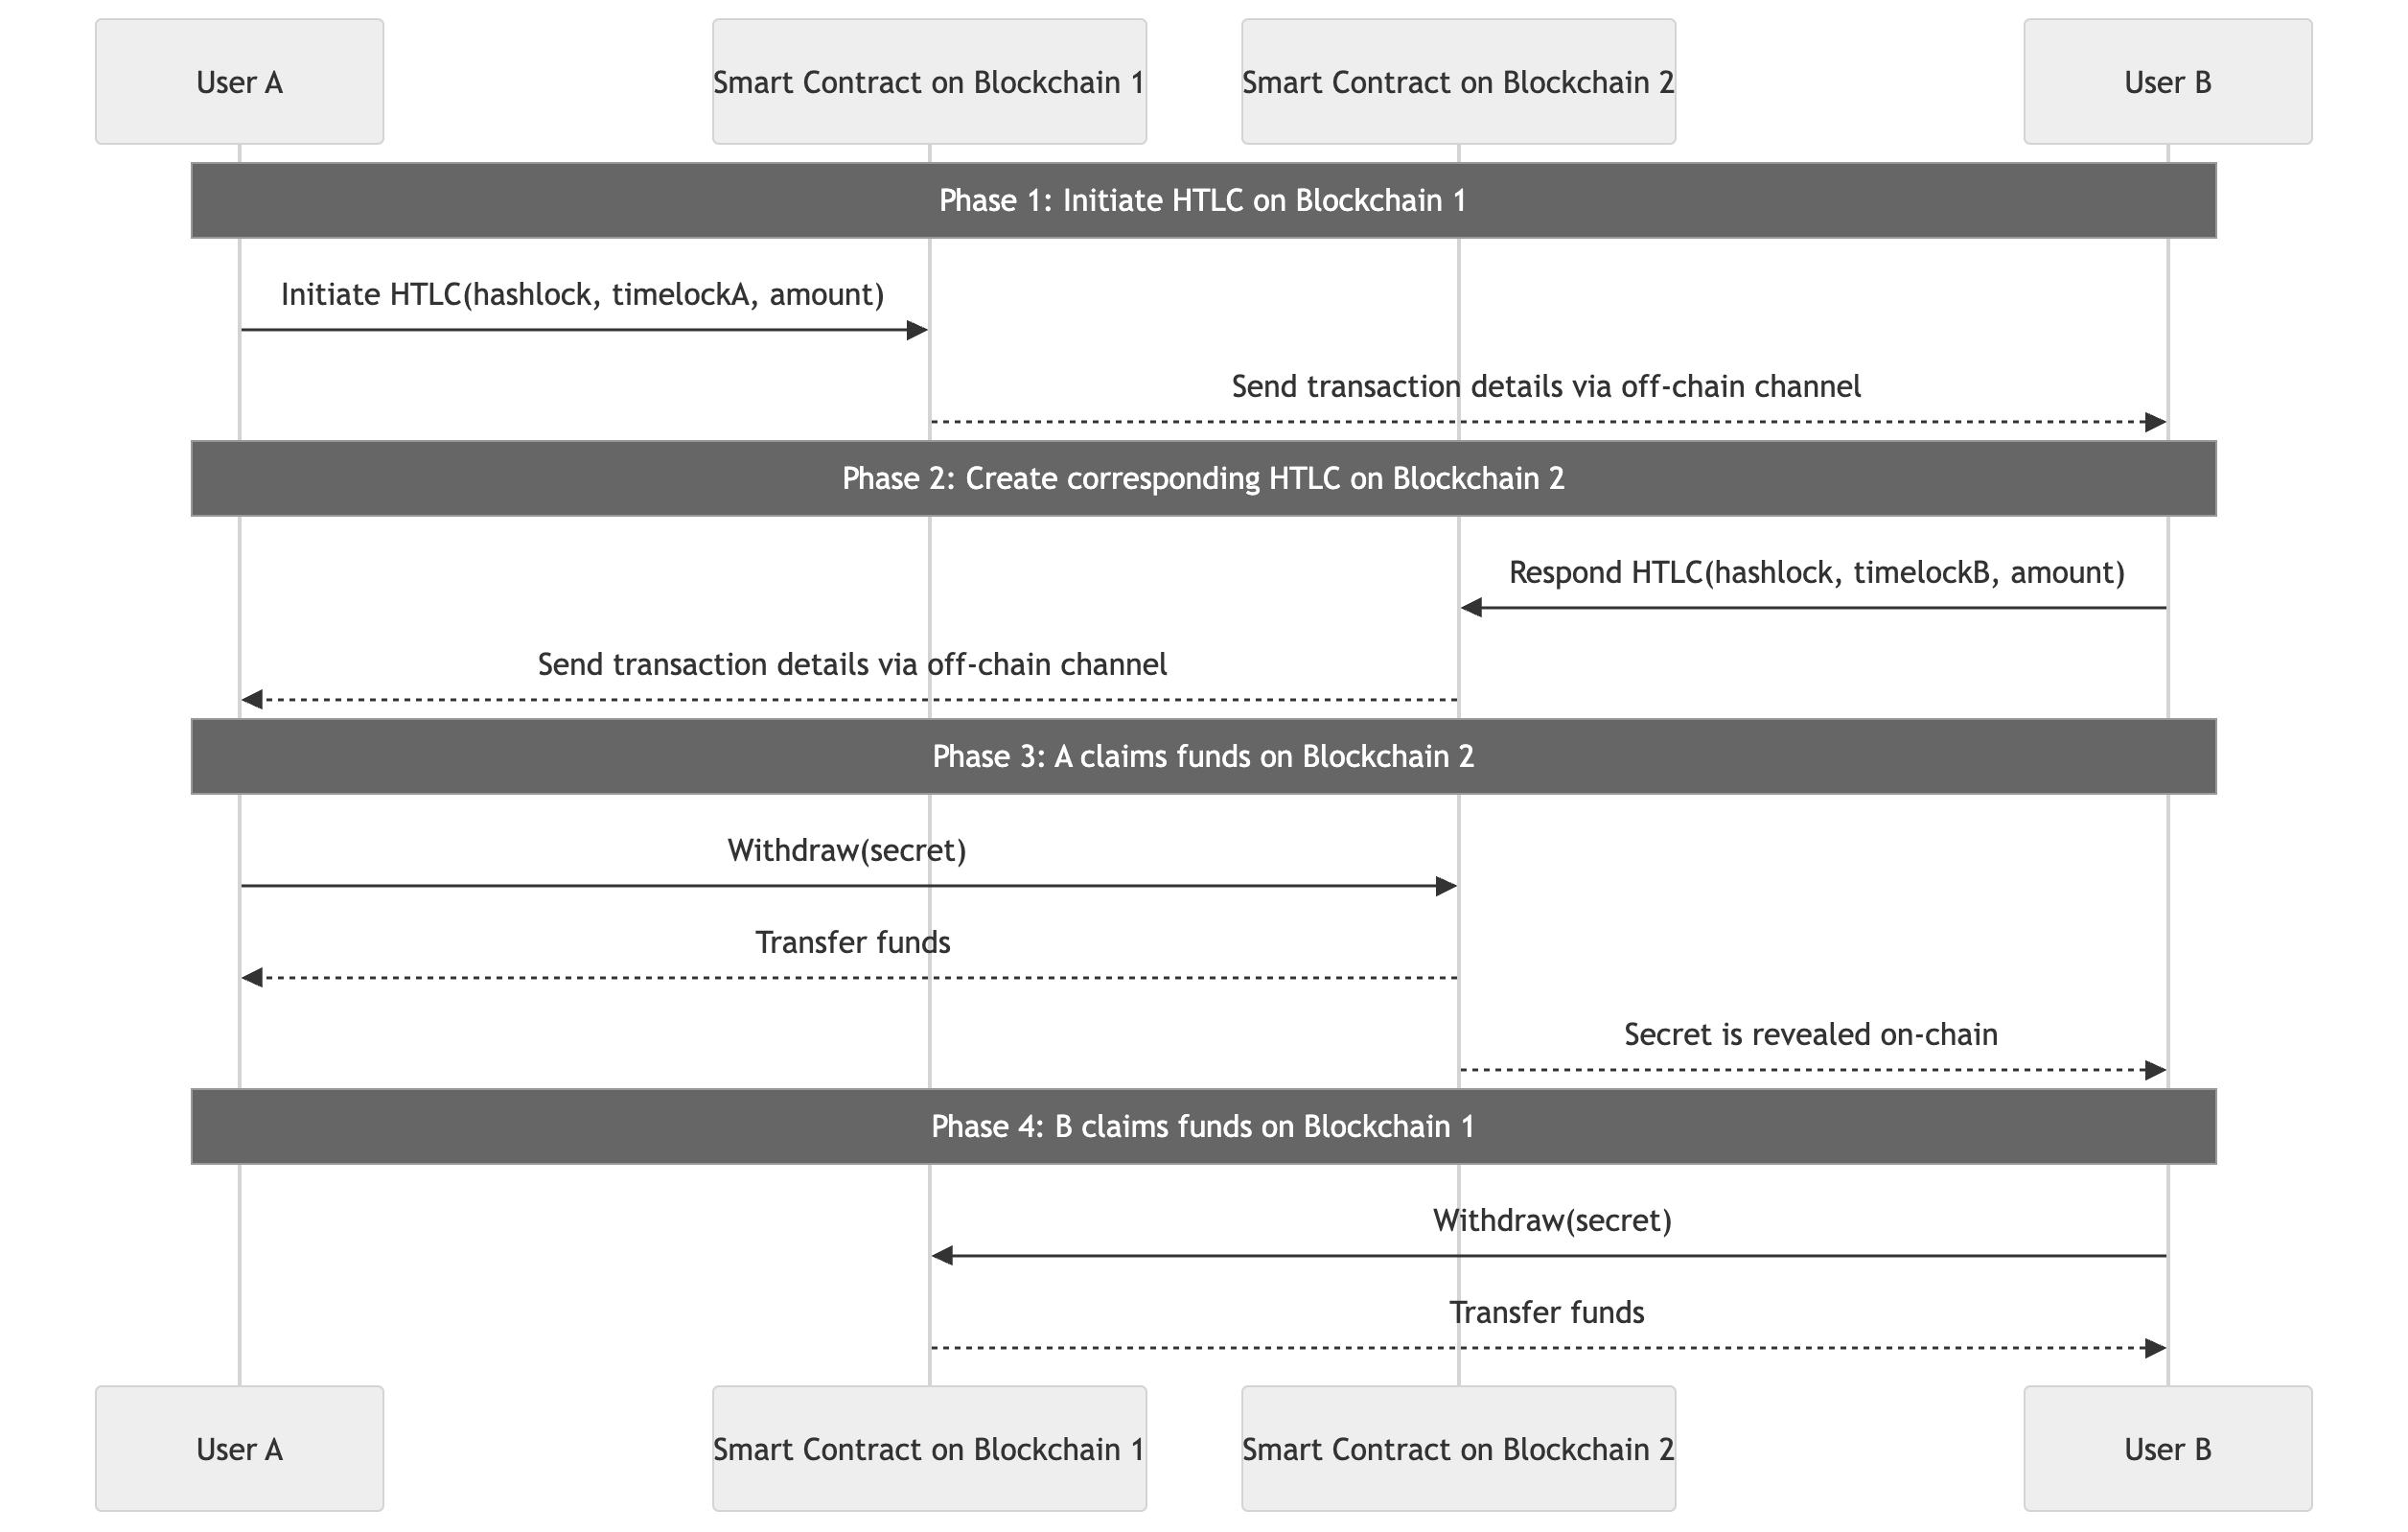
\includegraphics[width=\linewidth]{figures/c3/htlc-sequence}
  \end{center}
  \caption{Giao thức HTLC cho cross-chain atomic swap: 4 giai đoạn initiate, respond, claim A, claim B}
  \label{fig:htlc-sequence}
\end{figure}

Để đảm bảo tính nguyên tử (atomicity) và loại bỏ nhu cầu tin tưởng giữa các bên tham gia, hệ thống áp dụng cơ chế Hashed Timelock Contract (HTLC). Theo đó, mỗi bên sẽ khóa tài sản của mình vào một hợp đồng với cùng một giá trị hashlock. Giao dịch chỉ được hoàn tất khi một bên cung cấp đúng preimage tương ứng với hash đã cam kết. Nếu điều kiện này không được thỏa mãn trong khoảng thời gian quy định, toàn bộ giao dịch sẽ bị hoàn tác.

Việc sử dụng HTLC trong bối cảnh netting cho phép thực hiện các giao dịch cross-chain theo cách an toàn mà không cần trung gian. Đồng thời, nó đảm bảo rằng không có trường hợp thực thi một phần, tức là hoặc tất cả các bên đều nhận được tài sản như kỳ vọng, hoặc không bên nào bị thiệt hại. Đây là yếu tố quan trọng giúp Netting Layer duy trì được tính trust-minimized trong môi trường phi tập trung.

% TODO: Sequence diagram - end-to-end Netting Layer flow (intent submit -> match -> HTLC settle).
% Place image at figures/c3/netting-sequence.png and uncomment below.
% \begin{figure}[H]
%   \begin{center}
%   \includegraphics[width=\linewidth]{figures/c3/netting-sequence}
%   \end{center}
%   \caption{Biểu đồ tuần tự: luồng thực thi đầy đủ của Netting Layer}
%   \label{fig:netting-sequence}
% \end{figure}

\subsection{Intent Accelerator Layer}

Trong trường hợp Netting Layer không thể tìm được match trong một khoảng thời gian hợp lý, intent sẽ được chuyển sang Intent Accelerator Layer. Tại đây, intent được broadcast ra thị trường cho các solver, filler hoặc market maker, những thực thể có khả năng cung cấp thanh khoản và thực thi giao dịch một cách nhanh chóng. Cơ chế này giúp tăng đáng kể xác suất hoàn tất giao dịch, đặc biệt trong các tình huống thị trường không có đủ thanh khoản nội bộ.

Ưu điểm nổi bật của layer này là tốc độ thực thi cao, gần như tức thời, do tận dụng được thanh khoản sẵn có từ bên ngoài. Đồng thời, việc mở rộng ra thị trường giúp tăng khả năng match intent, từ đó cải thiện trải nghiệm người dùng. Tuy nhiên, chi phí thực thi sẽ cao hơn do phải trả incentive cho solver. Ngoài ra, hệ thống cũng phải đối mặt với các rủi ro liên quan đến hành vi chiến lược của các bên thứ ba, chẳng hạn như selective fill, sandwich logic hoặc việc solver từ chối tham gia nếu điều kiện không đủ hấp dẫn.

Một cải tiến quan trọng trong layer này là cơ chế incentive tăng dần theo thời gian, có thể được xem như một dạng Dutch auction. Thay vì yêu cầu người dùng trả phí cao ngay từ đầu, hệ thống thiết kế incentive như một hàm tăng theo thời gian. Ban đầu, incentive gần như bằng không và sẽ tăng dần cho đến một mức tối đa. Cơ chế này tạo ra một bài toán chiến lược cho solver, trong đó họ phải cân nhắc giữa việc thực thi sớm với phần thưởng thấp nhưng chắc chắn, hoặc chờ đợi để nhận phần thưởng cao hơn nhưng đối mặt với rủi ro mất cơ hội do solver khác hoặc do intent được match ở layer trước.

Cách tiếp cận này mang lại nhiều lợi ích quan trọng. Trước hết, nó giúp giảm thiểu việc người dùng phải trả phí quá cao trong những trường hợp không cần thiết. Đồng thời, nó tạo ra một môi trường cạnh tranh tự nhiên giữa các solver, buộc họ phải bộc lộ khả năng thực thi và mức độ chấp nhận rủi ro của mình. Về mặt cơ chế, đây là một thiết kế hiệu quả trong việc cân bằng giữa chi phí và tốc độ, đồng thời hạn chế các hành vi khai thác không công bằng.

% TODO: Sequence diagram - Intent Accelerator with Dutch auction (broadcast -> solver commit -> fill).
% Place image at figures/c3/accelerator-sequence.png and uncomment below.
% \begin{figure}[H]
%   \begin{center}
%   \includegraphics[width=\linewidth]{figures/c3/accelerator-sequence}
%   \end{center}
%   \caption{Biểu đồ tuần tự: Intent Accelerator Layer với cơ chế Dutch auction incentive}
%   \label{fig:accelerator-sequence}
% \end{figure}

\subsection{Fallback Bridge Aggregator}

Nếu cả Netting Layer và Intent Accelerator Layer đều không thể thực hiện intent, hệ thống sẽ chuyển sang lớp cuối cùng là Fallback Bridge Aggregator. Đây là lớp đảm bảo rằng giao dịch vẫn có thể được hoàn tất bằng cách sử dụng các bridge truyền thống hoặc các hệ thống thanh khoản bên ngoài. Mặc dù chi phí và độ phức tạp cao hơn, lớp này đóng vai trò quan trọng trong việc đảm bảo tính ổn định và độ tin cậy của toàn hệ thống.

Ưu điểm chính của Fallback Layer là khả năng đảm bảo completion gần như tuyệt đối, từ đó cải thiện trải nghiệm người dùng và giảm thiểu các trường hợp thất bại. Tuy nhiên, đổi lại, chi phí thực thi thường cao hơn do phải đi qua nhiều bước trung gian và phụ thuộc vào hạ tầng bên ngoài. Ngoài ra, execution path cũng dài hơn, làm tăng độ trễ và mức độ phức tạp trong việc theo dõi giao dịch.

Trong tổng thể kiến trúc, Fallback Bridge Aggregator đóng vai trò như một lớp bảo hiểm cuối cùng, đảm bảo rằng mọi intent đều có thể được thực hiện, ngay cả trong những điều kiện thị trường không thuận lợi. Nhờ đó, hệ thống đạt được sự cân bằng giữa hiệu quả và độ tin cậy, khi vừa tối ưu chi phí trong trường hợp lý tưởng, vừa đảm bảo khả năng hoàn tất trong mọi tình huống.

% TODO: Sequence diagram - Fallback bridge invocation (intent -> bridge adapter -> external bridge -> settle).
% Place image at figures/c3/fallback-sequence.png and uncomment below.
% \begin{figure}[H]
%   \begin{center}
%   \includegraphics[width=\linewidth]{figures/c3/fallback-sequence}
%   \end{center}
%   \caption{Biểu đồ tuần tự: Fallback Bridge Aggregator ủy thác qua bridge bên thứ ba}
%   \label{fig:fallback-sequence}
% \end{figure}

Tổng thể, kiến trúc ba lớp được trình bày trong chương này cho thấy một cách tiếp cận linh hoạt và hiệu quả đối với bài toán bridge dựa trên intent. Bằng việc kết hợp Netting Layer, Intent Accelerator Layer và Fallback Bridge Aggregator, hệ thống có thể thích nghi với nhiều điều kiện thị trường khác nhau, từ đó tối ưu hóa cả chi phí, tốc độ và độ tin cậy. Cách thiết kế này không chỉ cải thiện hiệu năng thực thi mà còn mở ra hướng phát triển mới cho các giao thức DeFi dựa trên intent, nơi quá trình execution trở thành một cơ chế động và có thể tối ưu theo thời gian thay vì cố định như trước đây.

\section{Mô hình dữ liệu}

\subsection{Các thực thể chính}

Mô hình dữ liệu của hệ thống xoay quanh các thực thể trung tâm sau:

\begin{itemize}
    \item \textbf{IntentOrder}: đơn vị nghiệp vụ chính, đại diện cho một intent của người dùng. Bao gồm \texttt{orderId}, \texttt{srcChain}, \texttt{desChain}, \texttt{amount} (số lượng USDC hiệu dụng), \texttt{incentiveFee} (tuỳ chọn), \texttt{deadline}, \texttt{userAddress}, và trường \texttt{status} thuộc tập \texttt{\{QUEUED, PARTIAL, MATCHED, EXPIRED\}}.
    \item \textbf{CycleMatch}: một chu trình bù trừ được tìm thấy bởi Matching Engine, gồm tập các \texttt{CycleMatchEntry} (mỗi entry là một intent tham gia với số lượng được khớp) và tổng \texttt{matchedAmount} của chu trình.
    \item \textbf{MatchedOrderEntry}: đại diện đóng góp của một intent trong một sự kiện matching, với \texttt{matchedAmount}, \texttt{remainingAmount} và trạng thái \texttt{MATCHED} hoặc \texttt{PARTIAL}.
    \item \textbf{MatchResult}: kết quả của một tick scheduler, gói toàn bộ các \texttt{MatchedOrderEntry} và \texttt{CycleMatch} phát sinh tại thời điểm đó.
    \item \textbf{ExecutionPlan}: lệnh thực thi được sinh ra từ một \texttt{MatchResult} hoặc từ kết quả Accelerator/Fallback, mô tả các bước on-chain cần thực hiện (initiate HTLC, claim, refund, gọi bridge ngoài).
\end{itemize}

% TODO: Class diagram - core domain entities and their relationships.
% Place image at figures/c3/class-diagram.png and uncomment below.
% \begin{figure}[H]
%   \begin{center}
%   \includegraphics[width=\linewidth]{figures/c3/class-diagram}
%   \end{center}
%   \caption{Biểu đồ lớp: mô hình dữ liệu nghiệp vụ trung tâm}
%   \label{fig:class-diagram}
% \end{figure}

\subsection{Lược đồ event log}

Trạng thái offchain được duy trì thông qua một event log dạng append-only đóng vai trò nguồn sự kiện duy nhất (single source of truth). Mỗi sự kiện đại diện cho một thay đổi trạng thái nguyên tử của hệ thống, ví dụ: \texttt{IntentSubmitted}, \texttt{IntentValidated}, \texttt{CycleMatched}, \texttt{HTLCInitiated}, \texttt{HTLCClaimed}, \texttt{HTLCRefunded}, \texttt{AcceleratorBroadcast}, \texttt{SolverCommitted}, \texttt{FallbackInvoked}, \texttt{IntentSettled}, \texttt{IntentExpired}. Các consumer downstream (Backend snapshot, Risk engine, Orderbook) đọc tuần tự log để dựng lại trạng thái phái sinh, đảm bảo tính nhất quán giữa các thành phần và cho phép replay khi cần phục hồi.
